\section{Optimization with Adaptive Density Control of 3D Gaussians}
\label{sec:opt-dens}


The core of our approach is the optimization step, which creates a dense set of 3D Gaussians accurately representing the scene for free-view synthesis.
In addition to positions $p$, $\alpha$, and covariance $\Sigma$, we also optimize SH coefficients representing color $c$ of each Gaussian to correctly capture the view-dependent appearance of the scene. 
The optimization of these parameters is interleaved with steps that control the density of the Gaussians to better represent the scene.


\subsection{Optimization}

The optimization is based on successive iterations of rendering and comparing the resulting image to the training views in the captured dataset. Inevitably, geometry may be incorrectly placed due to the ambiguities of 3D to 2D projection. Our optimization thus needs to be able to \emph{create} geometry and also \emph{destroy} or \emph{move} geometry if it has been incorrectly positioned. The quality of the parameters of the covariances of the 3D Gaussians is critical for the compactness of the representation since large homogeneous areas can be captured with a small number of large anisotropic Gaussians.

We use Stochastic Gradient Descent techniques for optimization, taking full advantage of standard GPU-accelerated frameworks\TODO{ADD pytorch ref}, and the ability to add custom CUDA kernels for some operations, following recent best practice~\cite{plenoxels,dvgo-cvpr2022}. In particular, our fast rasterization (see Sec.~\ref{sec:tile-raster}) is critical in the efficiency of our optimization, since it is the main computational bottleneck of the optimization.

We use a sigmoid activation function for $\alpha$ to constrain it in the $[0-1)$ range and obtain smooth gradients, and an exponential activation function for the scale of the covariance for similar reasons.




We estimate the initial covariance matrix as an isotropic Gaussian with axes
equal to the mean of the distance to the closest three points. 
We use a standard exponential decay scheduling technique similar to Plenoxels~\cite{plenoxels}, but for positions only. The loss function is $\mathcal{L}_1$ combined with a D-SSIM term:

\begin{equation}
	\mathcal{L} = (1 - \lambda) \mathcal{L}_1 + \lambda \mathcal{L_{\textrm{D-SSIM}}}
\end{equation}

We use $\lambda~=~0.2$ in all our tests.
We provide details of the learning schedule and other elements in Sec.~\ref{sec:impl}.




\subsection{Adaptive Control of Gaussians}
We start with the initial set of sparse points from SfM and then apply 
our method to adaptively control the \REMOVAL{density \Dg~}\CORRECTION{of the 3D Gaussians}{number of Gaussians and their density over unit volume}\footnote{Density \CORRECTION{\Dg~}{of Gaussians} should not be confused of course with density $\sigma$ in the NeRF literature.}, allowing us to go from an initial sparse set of Gaussians to a denser set that better represents the \CORRECTION{screen}{scene}, and with correct parameters. 
After optimization warm-up (see Sec.~\ref{sec:impl}), we densify every 100 iterations and remove any Gaussians that are essentially transparent, i.e., with $\alpha$ less than a threshold $\epsilon_{\alpha}$.

Our adaptive control of \CORRECTION{density \Dg~}{the Gaussians} needs to populate empty areas. It focuses on regions with missing geometric features (``under-reconstruction''), but also in regions where Gaussians cover large areas in the scene (which often correspond to ``over-reconstruction'').
\TODO{MAYBE ADD FIGURE (GK)}
We observe that both have \emph{large} view-space positional gradients.
Intuitively, this is likely because they correspond to regions that are not yet well reconstructed, and the optimization tries to move the Gaussians to correct this. 

Since both cases are good candidates for densification, \CORRECTION{so}{} we 
densify Gaussians with an average magnitude of view-space position gradients above a threshold~$\tau_{\textrm{pos}}$, which we set to $0.0002$ in our tests.

We next present details of this process, illustrated in Fig.~\ref{fig:density_control}.

\begin{figure}[!h]
	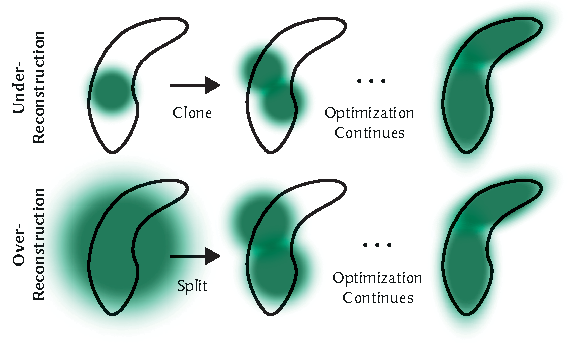
\includegraphics[width=\linewidth]{figures/density_control/density_control_01.pdf}
	\caption{
		\label{fig:density_control}
		Our adaptive Gaussian densification scheme.
		\emph{Top row (under-reconstruction)}: When small-scale geometry (black outline) is insufficiently covered, we clone the respective Gaussian.
		\emph{Bottom row (over-reconstruction)}: If small-scale geometry is represented by one large splat, we split it in two.
	}
\end{figure}

For small Gaussians that are in under-reconstructed regions, we need to cover the new geometry that must be created. 
For this, it is preferable to clone the Gaussians, by simply creating a copy of the same size, and moving it in the direction of the positional gradient.

On the other hand, large Gaussians in regions with high variance need to be split into smaller Gaussians. We replace such Gaussians by\REMOVAL{thus delete such Gaussians and introduce} two new ones\REMOVAL{Gaussians}, and divide their scale by a factor of $\phi~=~1.6$ which we determined experimentally.
We also initialize their position by 
using the original 3D Gaussian as a PDF for sampling.


In the first case we detect and treat the need for \CORRECTION{increasing the density \Dg}{increasing both the total volume of the system and the number of Gaussians}, while in the second case we conserve \CORRECTION{the total density \Dg~ of the system.}{total volume but increase the number of Gaussians.} 
\CORRECTION{Given that our problem is not strictly convex, the optimization sometimes can get stuck in local minima which may result in an unjustified increase in the Gaussian density.}{Similar to other volumetric representations, our optimization can get stuck with floaters close to the input cameras; in our case this may result in an unjustified increase in the Gaussian density.}
An effective way to moderate the increase in the number of Gaussians \CORRECTION{and to deal with the floaters} is to set the $\alpha$ value close to zero every $N=3000$ iterations. The optimization then increases the $\alpha$ for the Gaussians where this is needed while allowing our culling approach to remove Gaussians with $\alpha$ less than $\epsilon_{\alpha}$ as described above. \CORRECTION{We also}{Gaussians may shrink or grow and considerably overlap with others, but we periodically} remove \CORRECTION{}{Gaussians that are} very large \CORRECTION{Gaussians} in worldspace and \CORRECTION{Gaussians}{those} that have a big footprint in viewspace. This strategy results in overall good control over the total number of Gaussians. \ADDITION{The Gaussians in our model remain primitives in Euclidean space at all times; unlike other methods~\cite{barron2022mipnerf360,plenoxels}, we do not require space compaction, warping or projection strategies for distant or large Gaussians.}






